\cotefile{156-8}
\scanpage{2}
\unsure{AP|CP|CF} \uline{$\overline{\mathrm{VIII}}$}

\margin{Voir page \unsure{6|46}. \uline{\unsure{Def de morphisme}}}
% archive sheet number: 1

\scanpage{3}
\unsure{CF|CP} \uline{$\overline{\mathrm{VIII}}$}

% margin note written slanted, above the left branch
\margin{\uline{NB} Un magasin ``local'' \unsure{ce. qui|ce qui} \unsure{se réfère|réfère} à \deleted{\unsure{des}} \unsure{rels} \unsure{particulières} \unsure{d'incidence} aux \uline{lieux}.}

\diagram{
\begin{tikzcd}[ampersand replacement=\&,column sep=1em,row sep=2.6em,/tikz/scale=0.70,/tikz/transform shape]
\& \begin{gathered}
\text{\uline{Magasins généraux}}\\
M,\ \leq,\ \ll,\ |\circ|\\
\mathrm{Mag}\,1-\mathrm{Mag}\,4\ (\text{p.22})\\
\Sigma_M\subset\unsure{P|\mathcal P|\mathscr P}(M)
\end{gathered}\arrow[-,dl]\arrow[-,dr] \& \\
\begin{gathered}
\text{\uline{Magasins locaux}}\\
M,\ \leq,\ \overset{\circ}{\ll},\ |\circ|_{\unsure{\mathcal L|L}}\\
\mathrm{Magloc}\,1-\mathrm{Magloc}\,3\ (\text{p.23})\\
\Sigma_M\subsetP(\mathcal L)
\end{gathered}\arrow[-,dr,shift left=1.5pt]\arrow[-,dr,shift right=1.5pt]
\&\begin{gathered}(A,B\in\Sigma_M\\A\cap B=\varnothing\Longleftrightarrow A|\circ|B)\end{gathered}
\&\begin{gathered}
\text{\uline{Magasins \deleted{\unsure{transparents}}}}\\
\text{\inserted{(à Ombres) fidèles}}\\
M,\ \leq,\ \overset{\circ}{\ll}\\
\mathrm{Magfid}\,1-\mathrm{Magfid}\,2\ (\text{p.31})
\end{gathered}\arrow[-,dl]\arrow[-,d]\\
\&\begin{gathered}
\text{\uline{Magasins \deleted{ponctuels}}}\\
\text{\inserted{ponctuaires}}\\
M,\ \leq,\ \overset{\circ}{\ll}\\
\mathrm{Magponc}\,1-3\ (\text{p.24}).\\
\Sigma_M\simeqP(\mathcal L)
\end{gathered}\arrow[-,d]
\&\begin{gathered}
\text{\uline{Maquettes}}\\
M,\ \leq\\
\text{\uline{Maq}}\,1:\ \leq\ \text{rel. d'ordre}\ (\text{p.25})\\
\Sigma_M\simeqP(M)
\end{gathered}\\
\&\begin{gathered}
\text{\uline{Magasins ensemblistes}}\\
\mathcal L,\ M\subset\mathrm{Fig\acute{e}l}(\mathcal L)\\
\unsure{\mathrm{Magens}|\mathrm{Magun}}\,1,\ \mathrm{Magens}\,2\ (\text{p.9})
\end{gathered}\arrow[-,d]\&\\
\&\begin{gathered}
\text{\uline{Magasins \inserted{\uline{ensemblistes}} modérés}}\\
\mathcal L,\ M\subset\mathrm{Fig\acute{e}l}(\mathcal L)\\
\mathrm{Magens}\,1-\mathrm{Magens}\,3
\end{gathered}\&
\end{tikzcd}}

% margin note below the local-magasin node
\margin{(\unsure{cette} inclusion ne commute pas néc. à $A\cap B$ \unsure{ni|m.} (ni à $\varnothing$?), et encore moins : $\operatorname{Sup}(A,B)$}

% margin note left of the ponctuaire node; added wording is above the line
\margin{\figure{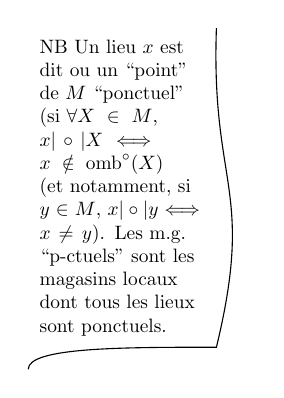
\begin{tikzpicture}[scale=0.7,transform shape]
\node[anchor=north west,align=left,text width=3cm,inner sep=0pt] (n) at (0,0) {\uline{NB} Un lieu $x$ est dit \inserted{\unsure{ou} un ``point'' de $M$} ``\uline{ponctuel}'' (\unsure{si} $\forall X\in M$, $x|\circ|X\Longleftrightarrow x\notin\mathrm{omb}^{\circ}(X)$ (et notamment, si $y\in M$, $x|\circ|y\Longleftrightarrow x\ne y$). Les \unsure{m.g.} ``\unsure{p-ctuels}'' sont les magasins locaux dont tous les lieux sont ponctuels.};
\draw ([xshift=2mm,yshift=2mm]n.north east) .. controls ([xshift=1mm]n.east) and ([xshift=9mm]n.east) .. ([xshift=2mm,yshift=-2mm]n.south east) .. controls ([yshift=-2mm]n.south) and ([xshift=-2mm,yshift=-2mm]n.south west) .. ([xshift=-2mm,yshift=-6mm]n.south west);
\end{tikzpicture}}}

% margin note to the right of the faithful-magasin branch, within a drawn enclosure
\margin{\figure{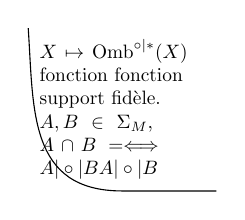
\begin{tikzpicture}[scale=0.7,transform shape]
\node[anchor=north west,align=left,text width=3cm,inner sep=0pt] (n) at (0,0) {$X\mapsto\mathrm{Omb}^{\unsure{\circ|*}}(X)$ \deleted{\unsure{fonction}} \unsure{fonction} support \uline{fidèle}. $A,B\in\Sigma_M$, $A\cap B=\varnothing\Longleftrightarrow\deleted{\unsure{A|\circ|B}}\inserted{A|\circ|B}$};
\draw ([xshift=-2mm,yshift=2mm]n.north west) .. controls ([xshift=-1mm]n.west) and ([xshift=-2mm,yshift=-2mm]n.south west) .. ([yshift=-2mm]n.south) -- ([xshift=2mm,yshift=-2mm]n.south east);
\end{tikzpicture}}}

% margin note right of Maquettes
\margin{(\uline{NB} Une maquette, \unsure{un|ou|est} espace \inserted{\unsure{ultra|ultraf.}} top. satisfaisant l'axiome de séparation $T_0$, n'est un magasin \deleted{local (avec \unsure{pour les éléments discrets|pour éléments les éléments discrets})} ponctuel que si elle est discrète.}

% margin note left of the ensembliste node
\margin{Ce \unsure{sont} les seuls magasins qui \deleted{\unsure{sont|soit}} correspondent aux \unsure{pts de vues} communément \unsure{admis} pour ``la topologie''}

% margin note left of the modere node
\margin{Correspondent à \deleted{des} ``topologies modérées'', qui n'ont été \unsure{développées} à présent que pour la seule structure linéaire par morceaux \unsure{sur} $\mathbb R$}

% margin note right of the modere node
\margin{NB Il y a des magasins modérés non ensemblistes, p. ex. les maquettes.}

\uline{NB} Je préfère finalement, dans $M$, noter $\unlhd$ la relation d'incidence, et noter de $\unsure{=|\simeq}$ la relation d'incidence entre $M$ et $F$. La notation $\triangleleft$ sera l'incidence stricte. La relation d'inclusion entre figures sera notée $\deleted{\unsure{\leq}}\subseteq$, \unsure{où n' confusion à craindre}, $\deleted{\unsure{\subseteq}}\leq$ (inclusion des figures). Je noterai $\overset{s}{\leq}$ pour les subdivisions \unsure{?}
% archive sheet number: 2

\scanpage{4}
% Faint reversed typescript is show-through from the other face of the sheet.
Multistrates orientés -- \uline{magasins \unsure{orienteurs}}

Données d'un magasin \unsure{orienteur} :
\[
M,\ \underset{\substack{\text{incidence}\\\text{immédiate}}}{\triangleleft},\ \overset{\circ}{\ll},\ |\circ|,\
\underset{\substack{\text{involution}\\\text{ss pt fixe}\\\text{``multistr. orienté opposé''}}}{\inserted{a:}\ X\mapsto X^-},\ M_0^+\deleted{\unsure{\subset M}}
\]

\uline{Magor. 1}\quad a) $\triangleleft$ antiréflexive. Le préordre strict engendré $<$ ($X<Y$ ssi $\exists\ X_0=X\mathrel{\triangleleft}X_1\mathrel{\triangleleft}\cdots\mathrel{\triangleleft}X_{n-1}\mathrel{\triangleleft}X_n\unsure{=|\leq=}Y$) est un ordre strict (pas de chaînes fermées, i.e. on ne peut avoir $X<X$). Il satisfait la condition des chaînes \deleted{\unsure{descendantes}} \inserted{\unsure{de longueur finie}}.

\deleted{tout élément est de dim. finie, et les éléments minimaux \unsure{qu'il majore|qui le majorent} \unsure{ont une certaine} \illegible{3} \unsure{dans lui}}

(en particulier, tout $X\in M$ de dim. finie pour $\leq$).

% margin note written slanted, down the left edge
\margin{\unsure{Ainsi} $\triangleleft$ \unsure{revient} à donner un ordre strict \unsure{vérifiant} la cond. des chaînes descendantes.}

b) $\overset{\circ}{\ll}$ relation d'ordre

c) $|\circ|$ \deleted{symétrique} antiréflexive.

d) $X\mapsto X^-$, involution sans pt fixe.

(e) $M_0^+$ est une partie de $M$.

(\uline{Magor $1'$} $\deleted{\unsure{\Longleftarrow}}$, (a) $X\triangleleft Y\Longrightarrow X^-\triangleleft Y^-$, $\deleted{\unsure{X\triangleleft Y^-}}$

b) $X\overset{\circ}{\ll}Y'\Longrightarrow X^-\overset{\circ}{\ll}Y^-$

c) $X|\circ|Y\Longrightarrow X^-|\circ|Y$.

\deleted{\unsure{d)}}

\margin{NB On peut avoir à la fois $X\triangleleft Y$ et $X\triangleleft Y^-$.}
\figure{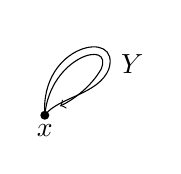
\begin{tikzpicture}[scale=0.65]
\fill (0,0) circle (2.5pt);
\draw (0,0) .. controls (-0.1,1.4) and (1.5,1.7) .. (1.25,0.9) .. controls (1.05,0.4) and (0.25,0.35) .. (0,0);
\draw[->] (0,0) .. controls (0.1,1.15) and (1.35,1.5) .. (1.1,0.9) .. controls (0.9,0.55) and (0.55,0.3) .. (0.3,0.18);
\node[below] at (0,0) {$x$};\node[right] at (1.3,1) {$Y$};
\end{tikzpicture}}

\uline{Magor 2}\quad a) Si $X,Y$ tels que $\exists Y'\quad X\overset{\circ}{\ll}Y'\leq Y$, alors $Y'$ \inserted{\unsure{unique}}

b) Si $X\overset{\circ}{\ll}Y$, et $X'\triangleleft X^{\unsure{\epsilon|\circ}}$, $\exists Y'\triangleleft Y$ avec
\[
X'\overset{\circ}{\ll}Y'
\]

\uline{Magor 3}\quad Si $X|\circ|Y$, et $X'\overset{\circ}{\ll}X$, $Y'\overset{\circ}{\ll}Y$, on a $X'|\circ|Y'$

-- \uline{Magor 4}\quad Si $X<Y$, alors $X|\circ|Y$.

\uline{Magor 6}\quad a) Soient $\unsure{Z|X}<X$, $\operatorname{codim}(\unsure{Y|Z},X)=2$. Alors il n'existe qu'\uline{un seul} $Y^{\unsure{\sharp|*}}$, avec $Z\triangleleft Y^{\sharp}\triangleleft X$, et de plus il existe $Y^{\unsure{\flat|b}}$ avec : $Z^-\triangleleft Y^{\flat}\triangleleft X^{\deleted{\unsure{-}}}$

b) Soit $X$ avec $\dim X=1$. Alors il existe et un seul $x\in M_0^+$, $x\triangleleft X$ \inserted{(i.e. $x\unsure{\in|=}M_0$)}

% A large marginal arrow points from Magor 5 to the space after Magor 4.
\margin{\figure{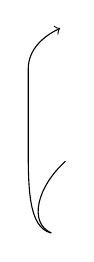
\begin{tikzpicture}[x=0.45cm,y=0.65cm]
\draw[->] (0,-4) .. controls (-0.65,-3.9) and (-0.65,-3.1) .. (-0.65,-2.3) -- (-0.65,-0.8) .. controls (-0.65,-0.4) and (-0.2,-0.15) .. (0.25,0);
\draw (0,-4) .. controls (-0.65,-3.8) and (-0.4,-3.1) .. (0.4,-2.6);
\end{tikzpicture}}}
\uline{Magor 5}\quad a) $x\in M_0^+\Longrightarrow\dim x=0$, i.e. $\overline{\exists}\ y$ avec $y\triangleleft x$.

b) On a $M_0=M_0^+\amalg a(M_0^+)$, i.e. \deleted{\unsure{x}} $x\in M_0^+\Longrightarrow x^-\notin M_0^+$, et $\forall x\in M_0$, on a $x\in M_0^+$ ou $x^-\in M_0^+$.
% archive sheet number: 3

\scanpage{5}
% The scan is upside down; text is transcribed in its own reading orientation.
\mspage{936 \deleted{quater} \handwritten{(iv)}}
% archive sheet number: 4

tions de texte (par rapport à l'édition provisoire d'Octobre dernier), chaque fois que j'ai trouvé que c'était plus simple que d'ajouter des notes de bas de page correctrices, et que cela ne modifiait pas de façon draconienne le sens et l'esprit du texte initial. J'ai enfin supprimé un passage d'une page et demie dans la sous-note ``Premiers ennuis - ou les caïds d'outre-Pacifique'' (\deleted{\unsure{In}} in ``La maffia'' n° $171_2$, (b)),\deleted{\unsure{mais pour}} en les remplaçant par un court commentaire rétrospectif.

\noindent\rule{2cm}{0.4pt}

Il est heureux que je n'aie pas suivi Mebkhout\deleted{\unsure{,}} pour donner à son contentieux avec Kashiwara une place qui ne lui revenait pas, dans \deleted{\unsure{le}} \handwritten{\inserted{mon}} compte-rendu de la mystification collective \inserted{sans précédent} qui a eu lieu autour de son oeuvre. Aussi je pense que les pages qui suivent, malgré les passages incorrects ou tendancieux (signalés en leur lieu) concernant le rôle et les mérites de Mebkhout, \deleted{\unsure{donnent|demeurent}} sont \handwritten{\inserted{pourtant}} un reflet circonstancié et fidèle d'un certain ``esprit du temps'' tel qu'il règne à présent (entre autres, sûrement) dans \deleted{\unsure{les}} \inserted{certains} milieux mathématiques, y compris parmi les plus huppés. \handwritten{\unsure{(}}Et ces deformations même dont je m'étais fait l'écho et la caution, m'apparaissent elles aussi comme un signe éloquent de cet esprit, dont mon ami Zoghman Mebkhout\deleted{\unsure{,}} \deleted{arrivé sur le tard} (j'ai fini par m'en rendre compte) \deleted{enfin)} est lui aussi,\deleted{un des produits} dans certains de ses réflexes et comportements, un produit.

\handwritten{(}171 (i)\handwritten{)}\quad L'ancêtre\quad (*)

(1 mars et 2-8 mai (1985)) \deleted{\unsure{(i)}} \deleted{\unsure{D}}\handwritten{D}ans chacune de ces ``quatre opérations'' partielles que \handwritten{\inserted{\unsure{j'ai}}} distinguées dans mon enterrement anticipé, c'est Deligne qui visiblement joue le rôle de chef d'orchestre (ou plutôt, de Grand Officiant aux

\noindent\rule{2cm}{0.4pt}

(*\deleted{\unsure{*}}) (13 mai) La présente note et les quatre suivantes formaient initialement une note unique, ``L'Apothéose'' (n° 171), du 1 mars. Elle incluait également la note précédente ``Les joyaux'' (n° 170(iii)). Elle a été reprise et considérablement étoffée entre les 2 et 8 mai, surtout en ce qui concerne la partie mathématique, et scindée en les quatre notes séparées ``L'ancêtre'', ``L'oeuvre...'', ``... et l'aubaine'', ``Le jour de gloire'' (n°s 171 (i) à (iv)), en plus de la note ``Les joyaux'' déjà mentionnée. Il s'y ajoutent les huit sous-notes (n°171 (v) à (xii)) se rapportant aux quatre notes en question, et les quatre sous-notes (n° $171_1$ à $171_4$) du mois d'avril, faisant le récit des étranges mésaventures de

\scanpage{6}
% Faint reversed typescript is show-through from the other face of the sheet.
\uline{Maquettes} \uline{\unsure{orienteuses|orienteurs}} : quand $X\overset{\circ}{\ll}Y\Longleftrightarrow X=Y$, $X|\circ|Y\Longleftrightarrow X\ne Y$.

\uline{Ex}\quad Les objets de $M$ sont de dim $\leq1$, $\overset{\circ}{\ll}=\mathrm{id}$, $x|\circ|y\Longleftrightarrow x\ne y$

\deleted{$M=M_0^+\unsure{\amalg}$}

On pose
\[
\begin{aligned}
M_0^+&=S\qquad\text{(``sommets'')}\\
M_1&=A\qquad\text{(``arcs'' \unsure{ou} ``arêtes orientées'')}
\end{aligned}
\]
On a involution sans points fixe $a$ sur $A$.

\deleted{On a} Par \unsure{Mag6 b|Magor6 b}, on a
\diagram{\begin{tikzcd}[ampersand replacement=\&]
A\arrow[r,"\sigma"]\& S
\end{tikzcd}}
[\unsure{donné|défini} par la condition]

Les maquettes orienteuses de dim \inserted{$\leq$}$1$ sont \uline{les} ``\uline{graphes}''.

\uline{NB}\quad Cette structure ne peut être décrite par une maquette, sauf quand il n'y a pas de \deleted{boucles fermées} \inserted{auto-boucles}.

\uline{Cas \inserted{des maquettes} de \deleted{\unsure{la}} dim 2}\quad Sauf erreur, on trouve la description des complexes cellulaires combinatoires de dim $\leq2$.
% archive sheet number: 5

\scanpage{7}
% The scan is upside down; text is transcribed in its own reading orientation.
\mspage{\handwritten{936 \deleted{\unsure{ter}} (iii)}}
% archive sheet number: 6
% margin note written slanted, beside the cancelled opening block
\margin{\handwritten{\unsure{note|not} b. de p.}}

\deleted{en parfaite conformité \inserted{en cela} avec l'esprit qui sévit \deleted{\unsure{dans jusque dans les}} à présent un peu partout dans le monde mathématique, et qui est \deleted{le seul dont il} celui surtout \deleted{\unsure{qu'il a eu devant ses yeux}} dont il a eu l'expérience dans son \deleted{travail} \handwritten{\inserted{milieu}} mathématique.}

\deleted{\unsure{Comme}} Ces déformations sont les plus flagrantes au niveau des démêlés de Mebkhout avec l'école japonaise d'analyse, et surtout \deleted{\unsure{avec}} \inserted{avec} Kashiwara, à qui il a voué une haîne violente, \deleted{qui touche} \handwritten{\inserted{touchant quasiment}} à l'obsession. Il y\deleted{\unsure{,}} a eu entre lui et Kashiwara un ``échange de mauvais procédés'', depuis 1976 semble-t-il, dont l'origine m'échappe. Mon texte de l'an dernier, comme de juste, ne fait état que des \deleted{coups} \handwritten{\inserted{``mauvais procédés''}} de \deleted{\unsure{Kashiwara|Kahiswara}}\unsure{Kahiswara|Kashiwara}, \deleted{et passe} \handwritten{\inserted{tout en passant}} sous silence presque totalement l'influence des idées de Kashiwara dans \deleted{son} l'oeuvre \inserted{de Mebkhout}, \deleted{et allant} \inserted{Mebkhout va} jusqu'à s'attribuer (``avec la meilleure foi du monde'', c'est une chose entendue) la paternité d'idées importantes dues à Kashiwara. Il semblerait que Kashiwara (en représailles peut-être) ne s'est pas fait faute de lui rendre la monnaie de sa pièce, en s'attribuant \inserted{\deleted{\handwritten{\unsure{et}}}(sans le mentionner)} des résultats \inserted{cruciaux} dûs à Mebkhout sans possibilité de doute.

Je me suis efforcé de rectifier les erreurs les plus flagrantes par des notes de bas de page\handwritten{\inserted{(*)}}, datées du 6,7 et 8 mai 1986. C'est là chose visiblement insuffisante, pour rectifier un ``éclairage'' d'ensemble qui, à présent, m'apparaît comme irréaliste: celui qui présente la nouvelle théorie des coéfficients comme étant, à peu de choses près, l'oeuvre \unsure{solitaire} du seul Zoghman Mebkhout. C'est pourquoi il m'a paru nécessaire d'ajouter \handwritten{\inserted{en plus,}} quelques pages de rétrospective critique, à la fin de l'Apothéose. Celles-ci complèteront également les commentaires dans le même sens que je fais dans l'\handwritten{``}Epilogue en Postscriptum\handwritten{''}\deleted{à la Lettre (\unsure{in ReS, Prélude en quatre}} (ReS \unsure{0|O} , Lettre, \deleted{\unsure{Post-Scriptum}} section 16 ``Amende honorable - ou l'esprit du temps (2)''), et les excuses publiques que j'y présente à Kashiwara, pour une présentation tendancieuse des faits\handwritten{,} dont je m'étais fait caution \handwritten{\inserted{sans réserve}}.

Il est assez clair pour moi que cette haîne violente vouée par mon ami Zoghman Mebkhout à un lointain Kashiwara, a été pour lui une diversion bienvenue, pour éviter de se confronter à une réalité autrement plus proche et autrement plus pénible. Car l'enterrement de Mebkhout, le continuateur \inserted{impénitent} de Grothendieck, n'a pas été l'oeuvre d'une lointaine école \deleted{j}\handwritten{j}aponaise (si ce n'est très accessoirement). Cet enterrement,\deleted{\unsure{a été l'oeuvre}} culminant en le ``happening'' incroyable d'un ``Colloque Pervers'', s'est fait \uline{ici} \uline{même}, \handwritten{\inserted{\unsure{Il|Je} a été}} orchestré par les élèves de \deleted{l'}\handwritten{\inserted{cet}} ``ancêtre'' dont \deleted{il} \handwritten{\inserted{Mebkhout}} s'inspirait \deleted{ouvertement} publiquement - par ceux-là même, \deleted{donc,} qu'il considérait comme ``les siens''. \deleted{Il} \handwritten{\inserted{Mebkhout}} a été trahi par ceux-là même qu'il admirait \handwritten{\inserted{sans réserve}}, et en qui il avait toute confiance.

\noindent\rule{3cm}{0.4pt}

\handwritten{(*)} Exceptionnellement, j'ai aussi fait ici et là quelques menues correc-

\scanpage{8}
\mspage{1}
CF \uline{$\overline{\mathrm{VIII}}$}

\uline{Analysis Situs} (quatrième mouture)

% margin note written slanted
\margin{26. juin 86}

\textcircled{I}\quad\uline{Récapitulation en termes de ``magasins''.}

Je reprends la formalisation algébrique d'une ``algèbre de multistrates'', en ``magasin'' (de multistrates, magasin ``\unsure{fournisseur}'' de ``matériaux''). La structure est celle d'un ens. $M$ avec trois relations
\[
\leq\qquad\ll,\quad|\circ|
\]
satisfaisant (cf CF \uline{$\overline{\mathrm{VII}}$}, p.\unsure{110}).

\uline{Mag 1}\quad a) $X\leq Y$ et $X\ll Y$ sont des relations d'\uline{ordre}, et \inserted{b)}
\[
X\leq Y\Longrightarrow X\ll Y
\]

\inserted{Si $X\in M$, on pose $\widetilde X=M_{\leq X}=\{Y\in M\mid Y\leq\unsure{x|X}\}$}

\uline{Mag 2}\quad $\forall X,Y$ avec $X\ll Y$, l'ens
\[
\widetilde Y^X=\{Z\in\widetilde Y\mid X\ll Z\}
\]
admet un plus petit élément.

\inserted{On écrit $X\overset{\circ}{\ll}Y$ quand cet élément est $Y$ lui$=$, i.e. $\widetilde Y^X$ \unsure{réduit} à $\{Y\}$.}

\uline{Mag 3}\quad\textcircled{a} $X|\circ|Y$ est symétrique et antiréflexive, i.e. $X|\circ|Y$ implique $Y|\circ|X$ et $X\ne Y$. \textcircled{b} De plus
\[
X|\circ|Y,\ X'\overset{\circ}{\ll}X,\ Y'\overset{\circ}{\ll}Y\Longrightarrow X'|\circ|Y'
\]

\uline{Mag 4}\quad Si $Y,Z\leq X$, \deleted{alors} $Y\ne Z$, alors $Y|\circ|Z$.

% margin note written slanted
\margin{\uline{NB} Cela \unsure{établit|évite} élégamment l'axiome \unsure{AtL3|At3}}

\uline{Définitions}\quad Pour $X,Y\in M$, on pose
\[
\begin{aligned}
X\mathrel{\unsure{\asymp|\bowtie|\gtrless}}Y
&\overset{\mathrm{def}}{\Longleftrightarrow}
\forall\unsure{x'|X'}\in\widetilde X\setminus\widetilde X\cap\widetilde Y,\quad
\unsure{y'|Y'}\in\widetilde Y\setminus\widetilde X\cap\widetilde Y,\ \text{on a}\quad\unsure{\widehat{x}'|x'}|\circ|y'\\
X\parallel Y&\overset{\mathrm{def}}{\Longleftrightarrow}
\forall x'\in\widetilde X,\ y'\in\widetilde Y,\ \text{on a}\quad X'|\circ|Y'.
\end{aligned}
\]

Donc
\[
X\parallel Y\Longleftrightarrow X\asymp Y,\ \text{et}\quad\widetilde X\cap\widetilde Y=\varnothing
\quad\text{(i.e. $\{X,Y\}$ \unsure{non} \unsure{minoré} pour $\leq$)}
\]
% archive sheet number: 8

\scanpage{9}
\mspage{2}
% margin note written slanted, upper left
\margin{Voir p. \unsure{90|9} \unsure{1bis}, 2bis, à mettre \unsure{avant|au v.} \unsure{les notes|les suites|leur suite} sur les figures.}

On appelle \uline{figure} \inserted{(inconditionnelle)} d'un magasin, un élément de l'ens
\[
\unsure{\mathcal F|\mathscr F}_M=\{\unsure{\Phi|\varphi}\subset M\mid\Phi\ \text{fermé dans $M$ pour}\ \leq,\ \text{et}\ \forall X,Y\in\Phi,\ \text{on a}\ X\mathrel{\unsure{\asymp|\bowtie|\gtrless}}Y\}
\]
L'ens $\mathcal F_M$ est l'ensemble des ``figures inconditionnelles'' (ou ``figures'' tout court) du magasin.

% margin note written slanted, left of the preceding paragraph
\margin{$\mathcal F_M$ sera appelé \uline{\unsure{Nablien|Nablium|Nablum}} \uline{\unsure{universel}} associé au magasin $M$.}

On sera amené, à l'occasion, de faire sur les figures envisagées deux types possibles de restrictions

1°) Conditions du type ``finitude'' ou ``locale finitude''.

\deleted{\unsure{sur les}}

2°) Condition restrictive ``polyédrale'' : si $X,Y\in\Phi$ et $\widetilde X\cap\widetilde Y\ne\varnothing$, on veut qu'il \deleted{$\widetilde X\cap\widetilde Y$} admette un plus grand élément, i.e. soit de la forme $\widetilde Z$, ou encore que $\operatorname{Inf}(X,Y)$ existe.

On étend à $\mathcal F$ les relations d'ordre $\leq$ et $\ll$ de $M$ (en plongeant $M$ dans $\mathcal F$ via les ``figures élémentaires'' $\widetilde X$, $X\in M$
\diagram{\begin{tikzcd}[ampersand replacement=\&]
M\arrow[r,hook]\&\mathcal F_M
\end{tikzcd}}
\[
\deleted{\unsure{\widetilde{\vphantom X}}}X\mathrel{\unsure{\mapstochar\relbar\relbar\bullet|\longmapsto}}\widetilde X=M_{\leq X}\qquad-
\]
\unsure{souvent} et par abus de langage, on identifie $M$ à \unsure{l'ens} des figures élémentaires, $X\in M$ : la figure élémentaire associée...)

% margin note written slanted, down the lower left edge
\margin{\unsure{Dans ce qui suit} on \unsure{désidentifiera} les figures d'avec les parties de $M$ qui les définissent, et pour une figure $F$ \unsure{désormais}, on \unsure{identifiera|identifie|désignera} la partie correspondante $\widetilde F=\{X\in M(\unsure{\subset|\in}\mathcal F)\mid X\leq F\}$.}

Donc
\[
F\leq G\overset{\mathrm{def}}{\Longleftrightarrow}F\subset G
\]
\[
\begin{aligned}
\text{NB le Sup des $F$ pour $\leq$ est}\quad&\bigcup\quad\text{dans $\unsure{P|\mathcal P|\mathscr P}(M)$}\\
\text{le Inf}\quad\underline{\hspace{3.3cm}}\quad&\bigcap\quad\underline{\hspace{2cm}}
\end{aligned}
\]
\[
F\ll G\overset{\mathrm{def}}{\Longleftrightarrow}\forall\unsure{x|X}\in\widetilde F,\ \exists Y\in\widetilde G,\ \text{avec}\ X\ll Y
\]
\[
\begin{aligned}
F\asymp G&\Longleftrightarrow\forall X\in\widetilde F,\ Y\in\widetilde G,\ \text{on a :}\ X\asymp Y\\
&\Longleftrightarrow\{F,G\}\ \text{majoré dans}\ \mathcal F\\
&\Longleftrightarrow\operatorname{Sup}(F,G)\ \text{existe dans}\ \mathcal F\ \deleted{\unsure{\text{(et }F\cup G\text{)}}}\\
&\Longleftrightarrow F\cup G\in\mathcal F
\end{aligned}
\]
% archive sheet number: 9
